
\subsubsection*{1. Uso cotidiano de la PC}
Utilizo mi PC principalmente para jugar videojuegos, tanto singleplayer como multiplayer. Me interesa obtener una buena experiencia visual y de fluidez, así como minimizar la latencia. También presto atención al rendimiento térmico y a la estabilidad del sistema durante sesiones largas de juego. El sistema operativo es Windows, y utilizo herramientas como MSI Afterburner y GeForce Experience.

\subsubsection*{2. Tareas y benchmarks representativos}

A continuación se presenta una tabla con distintos aspectos del gaming y los benchmarks o herramientas que mejor los representan.

\begin{center}
\begin{tabular}{|p{7cm}|p{7cm}|}
\hline
\textbf{Tarea / Escenario} & \textbf{Benchmarks} \\
\hline
Jugar videojuegos (rendimiento FPS y calidad gráfica) & Benchmarks sintéticos de GPU como \textbf{3DMark} \\
\hline
Jugar videojuegos (latencia) & Para latencia de entrada: \textbf{NVIDIA Reflex} (si es compatible con el juego) o herramientas como \textbf{CapFrameX} para analizar frame times. Para latencia de red: pruebas de ping y jitter a servidores de juego o valores integrados en juegos online. \\
\hline
\end{tabular}
\end{center}

\subsubsection*{3. Análisis de prueba con 3DMark}

Se realizó una prueba con la herramienta 3DMark para evaluar el rendimiento de la GPU y la CPU durante una carga gráfica sostenida.

\begin{itemize}
  \item \textbf{GPU:} NVIDIA GeForce GTX 1050 Ti
  \item \textbf{CPU:} Intel Core i3-9100F
  \item \textbf{Resolución:} 1920×1080
  \item \textbf{Sistema operativo:} Windows 10
\end{itemize}

Durante la prueba, se observaron los siguientes comportamientos:

\begin{itemize}
  \item La \textbf{GPU se mantuvo al 100\% de carga} durante toda la ejecución del test, lo que indica que es el principal limitante de rendimiento en este sistema.
  \item Se registró una temperatura promedio de \textbf{59.34°C} en la GPU, dentro de valores normales para este tipo de uso.
  \item La \textbf{CPU tuvo una carga media del 65\%}, lo cual indica que no está siendo un cuello de botella en este escenario particular.
  \item El \textbf{framerate promedio fue de 20 FPS}, lo que indica que el sistema puede ejecutar cargas gráficas intensas, pero con una fluidez limitada. Para juegos exigentes, es recomendable usar configuraciones gráficas medias o bajas para mantener los 60 FPS.
\end{itemize}

\hspace*{-1.2cm}
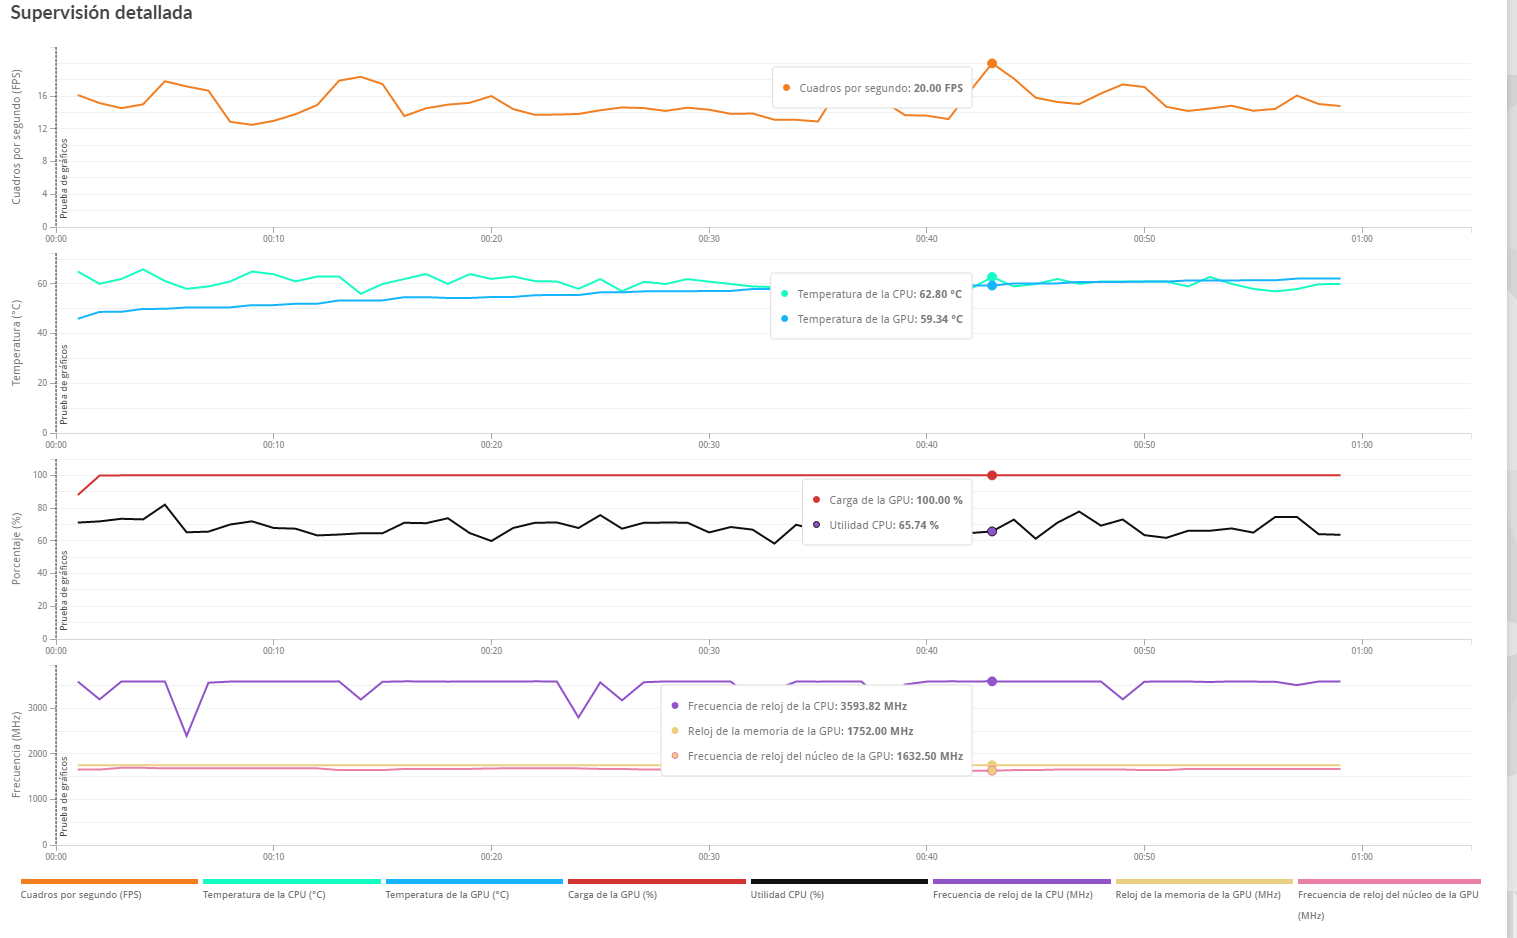
\includegraphics[width=1.2\textwidth]{img/3dmarkagu.png}

\begin{center}
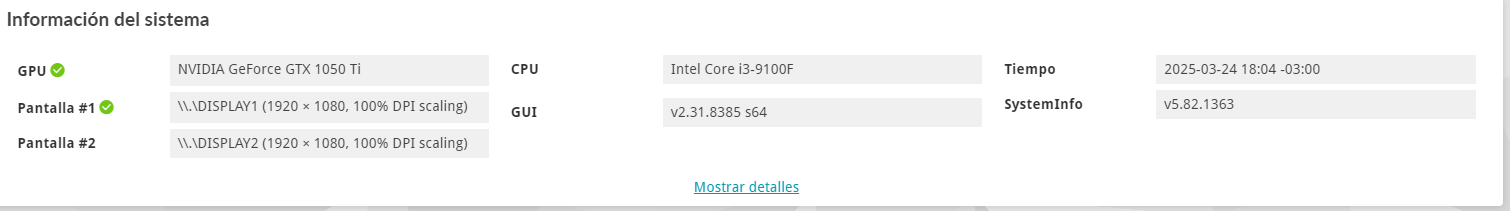
\includegraphics[width=1.1\textwidth]{img/informacionpcagu.png}
\end{center}

Este resultado es útil como línea base para comparar futuros upgrades. Si se busca mejorar el rendimiento en juegos, el cambio más impactante sería actualizar la GPU.

\subsubsection*{5. Medición de latencia de red con PingPlotter}

Para analizar la latencia de red, se utilizó la herramienta \textbf{PingPlotter}, apuntando al servidor de Riot Games (\texttt{riotgames.com}). Esta herramienta permite visualizar el comportamiento de la conexión en cada salto hasta el destino final, incluyendo pérdida de paquetes (packet loss), tiempo de ida y vuelta (ping) y jitter.

\begin{itemize}
  \item \textbf{IP objetivo:} 104.104.37.123
  \item \textbf{Duración de la prueba:} 10 minutos
  \item \textbf{Promedio de latencia:} 20.7 ms
  \item \textbf{Mínimo:} 14.0 ms \hspace{1cm} \textbf{Máximo (Cur):} 16.3 ms
  \item \textbf{Pérdida de paquetes:} Se observa pérdida parcial en los primeros saltos, pero no afecta al destino final.
\end{itemize}

La siguiente imagen muestra los resultados detallados de la prueba:

\begin{center}
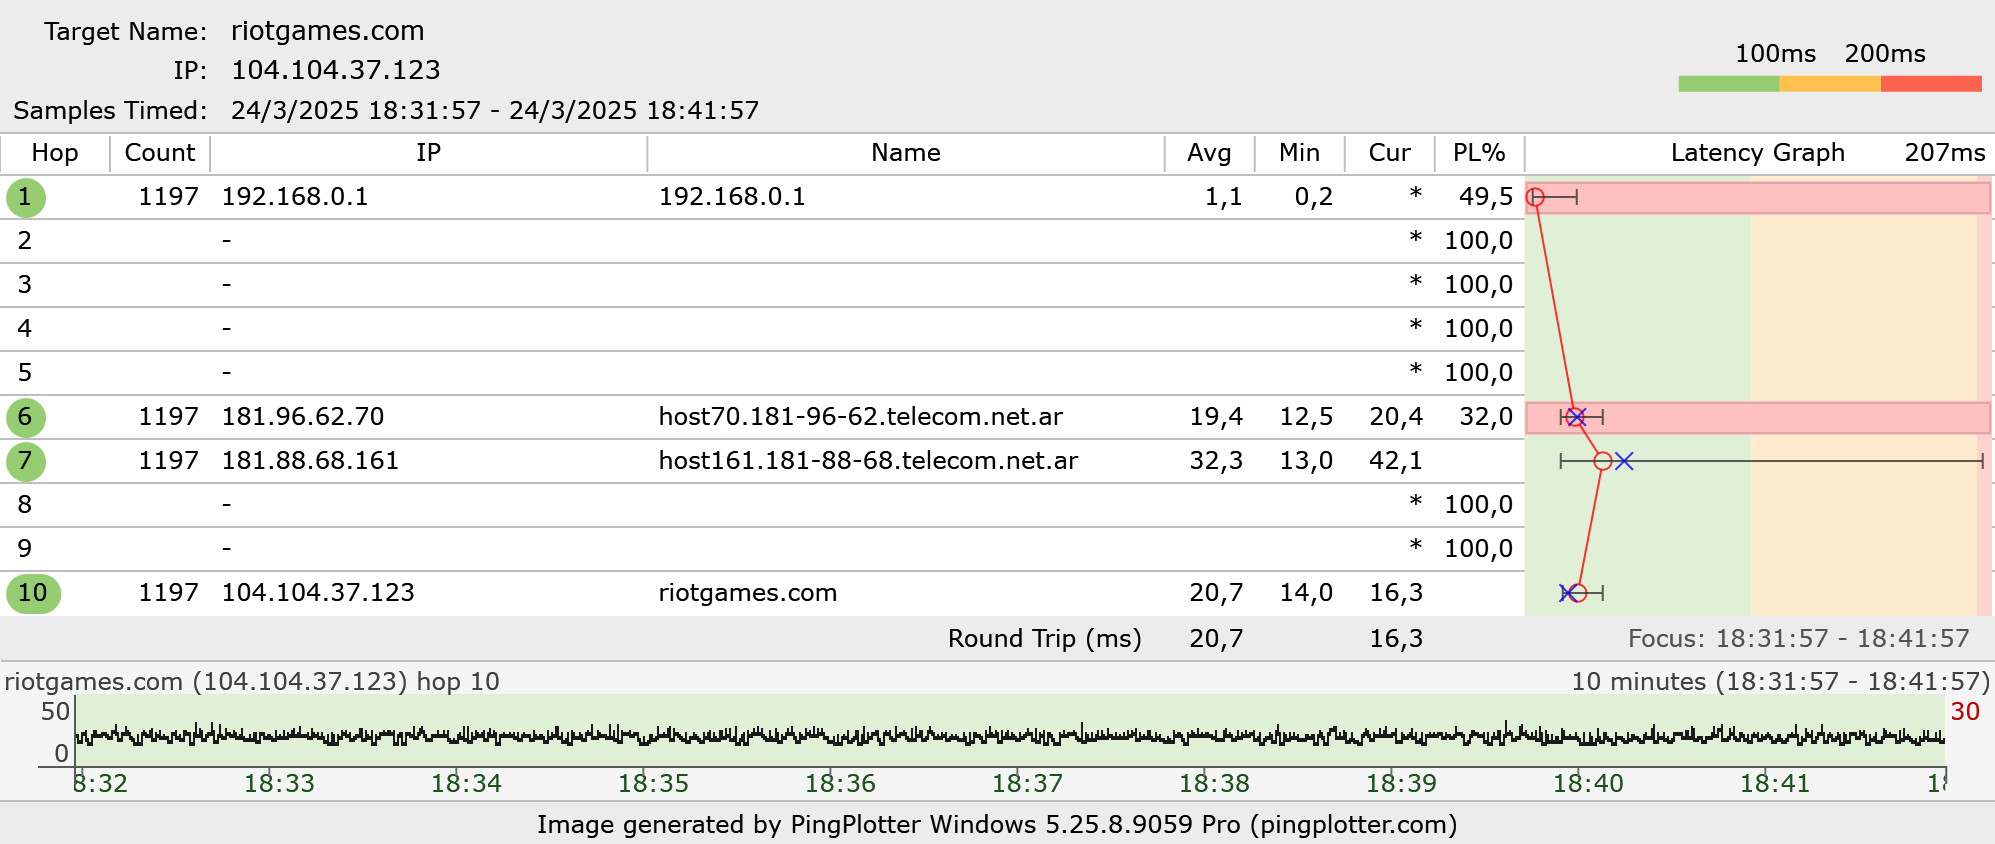
\includegraphics[width=1.05\textwidth]{img/latenciaagu.png}
\end{center}

Se observa que el \textbf{servidor de Riot Games responde con una latencia baja y estable}, lo cual es ideal para juegos en línea. La pérdida de paquetes en los primeros nodos suele deberse a equipos intermedios que priorizan tráfico real y no responden todos los pings; no representa un problema si no llega al destino final.

Este tipo de prueba resulta útil para identificar problemas de red, detectar cuellos de botella en la conexión o diferenciar si el lag en el juego proviene del servidor o del proveedor de internet.


\subsubsection*{4. Reflexión final}
En mi uso cotidiano, los benchmarks de GPU son los más representativos ya que reflejan el rendimiento en juegos reales. Herramientas como 3DMark me permiten comparar mi PC con otros equipos, y benchmarks integrados en juegos ayudan a medir rendimiento en contextos más prácticos. La latencia también es importante, sobre todo en juegos competitivos. Mi sistema rinde bien, pero siempre busco optimizar calidad gráfica sin comprometer fluidez.
